\documentclass[../thesis.tex]{subfiles}
% !TeX spellcheck = fr_FR

\begin{document}
    \chapter{Conclusion Générale}
    %\textcolor{red}{Il faut (je pense) revenir au sujet du challenge ROSE
    %	Système de reconnaissance des cultures et des mauvaises herbes basé sur l'apprentissage profond pour une pulvérisation ultra-localisée
    %	Perspective (ouvrir le sujet) : apport du Deep Learning, agriculture numérique : compatalibilité vers la transition agroécologique ? nouvelles possibilités ?
    %}
    
    % Comment trouver les meilleures critères pour discriminer les plantes ?  
    
    Les travaux de recherche de cette thèse ont été entrepris dans le cadre du projet européen \textit{H2020 IWMPRAISE}, dans le but de proposer des outils pour une meilleure gestion des adventices avec pour principal objectif de diminuer l'utilisation des produits phytosanitaires et leurs impacts écologiques (présentés dans l'introduction). Cette thèse, s'est aussi insérée dans l'\textit{ANR Challenge RoSE}, dont l'objectif était de mobiliser et d'évaluer les performances de différentes équipes de recherche, pour le désherbage de l'intra-rang en grandes cultures et cultures légumières de plein champ. % Cette évaluation couvre les différentes étapes liées à cette tâche, c'est-à-dire la détection, l'interprétation, la décision et l'action.
    
    Les recherches qui ont été effectuées et présentées dans ce manuscrit, concernent la tâche de détection des adventices, qui constitue encore aujourd'hui un verrou scientifique. Pour répondre aux autres tâches évaluées dans le cadre de l'\textit{ANR Challenge RoSE} (telles que l'interprétation, la décision et l'action), un partenariat avec la société \textit{SITIA}, les chambres d'Agriculture de Bretagne et Pays de Loire, et l'\textit{IRSEEM-ESIGELEC} a été établi en amont de cette thèse. L'ensemble constitue le consortium \textit{ROSEAU}. Ainsi, les résultats de ces recherches ont  vocation à être implémentés sur le robot \og TREKTOR \fg, de la société \textit{SITIA}, pour une gestion automatisée des adventices.
    
    %Pour répondre à la tâche de détection, il existe deux grande voie possible. Soit utiliser des algorithmes standards, souvent peu fiable. Soit util
    %La démarche envisagée c'est inscrit dans le domaine de l'agriculture numérique à travers une évaluation multi-critères des adventices détectées par imagerie pour une gestion localisée. 
    
    % JE N'ACCROCHE PAS AVEC CE PARAGRAPHE DONC JE PROPOSE AUTRE CHOSE
    % Tout au long de ce manuscrit, nous avons ainsi proposé des méthodes pour répondre à la problématique de détection des adventices. Elles reposent essentiellement sur des méthodes d'analyse d'image. On rappelle que l'objectif principal de cette thèse est de définir les ``meilleurs'' critères extractibles à partir d'images multispectrales, afin de discriminer les cultures des adventices. Cependant, étant donné que cette thèse s'insère dans le Challenge RoSE, d'autres méthodes ont été mises en œuvre afin de détecter les adventices en amont de l'extraction de critères. 
    
    L'objectif principal de cette thèse était de définir les ``meilleurs'' critères extractibles à partir d'images multispectrales, afin de discriminer les cultures des adventices. Toutefois, il est rapidement apparu que l'extraction et l'évaluation de critères ne présentaient pas de verrou scientifique majeur, mais que la performance et la stabilité des critères de discrimination dépendait de la segmentation des images. Ainsi, le travail s'est orienté vers la définition d'indices de végétation optimaux et d'une méthode de segmentation sémantique des instances à l'échelle de la feuille. La performance des méthodes proposées a été évaluée sur des images de feuillage dense, acquises en lumière naturelle. Au final, l'approche proposée mixe classification usuelle et apprentissage profond. 
    
    \newpage
    \section{Contributions}
    
    Comme évoqué dans le chapitre \ref{chap:computer-vision}, il existe deux grandes voies pour détecter les adventices : une approche standard d'analyse d'image ou l'utilisation du ``tout'' deep-learning. Notre méthode repose sur une architecture ``standard'' dont chaque partie a été améliorée par optimisation des hyperparamètres ou par apprentissage profond. La figure \ref{fig:09-global-view} ci-dessous, montre l'architecture finale qui a été développée ici.
    
    \begin{figure}[H]
        \centering
        \vspace{-2em}
        \tikzset{
	ppblock/.style={
		rectangle,
		minimum size=6mm,
		very thick,
		draw=black!50,
		text centered,
		font=\ttfamily,
		minimum width=8em,
		minimum height=6mm,
		top color=white,
	},
	%
	figure/.style={
		rectangle,
		rectangle split,
		rectangle split parts=2,
		very thick,
		draw=black!50,
		text centered,
		append after command={
			\pgfextra
			\fill[top color=#1, bottom color=#1]
			(\tikzlastnode.one west) 
			[rounded corners] |- (\tikzlastnode.north) -| (\tikzlastnode.one east) 
			[sharp corners]   |- (\tikzlastnode.one split) -| cycle;
			\fill[top color=white, bottom color=#1]
			(\tikzlastnode.two west) 
			[rounded corners] |- (\tikzlastnode.south) -| (\tikzlastnode.two east)  
			[sharp corners]   |- (\tikzlastnode.one split) -| cycle;
			\endpgfextra
		},
	},
    splitted/.style={
        rectangle,
        rectangle split,
        rectangle split horizontal,
        rectangle split parts=2,
        very thick,
        draw=black!50,
        text centered,
        append after command={
            \pgfextra
            \fill[top color=white, bottom color=#1]
            (\tikzlastnode.south)
            [rounded corners] -| (\tikzlastnode.west) |- (\tikzlastnode.one north)
            [sharp corners]   -| (\tikzlastnode.one split) |- cycle;
            \fill[top color=white, bottom color=#1]
            (\tikzlastnode.two south)
            [rounded corners] -| (\tikzlastnode.east) |- (\tikzlastnode.north)
            [sharp corners]   -| (\tikzlastnode.one split) |- cycle;
            \endpgfextra
        },
    },
	%
	static/.style={ppblock, bottom color={black!20}},
	nonterminal/.style={ppblock, bottom color={blue!30}},
	terminal/.style={ppblock, bottom color={green!20}},
	algorithm/.style={ppblock, bottom color={yellow!50}},
	error/.style={ppblock, bottom color={red!20}},
	type/.style={ppblock, bottom color={red!20}},
	loss/.style={ppblock, dashed, bottom color={black!20}, font=\itshape},
	%
	tiny/.style={
		rounded rectangle,
		very thick,
		draw=black!50,
		top color=white,
		bottom color=red!20,
        text centered,
		font=\ttfamily,
	},
    operator/.style = {
        circle,
        scale=0.6,
        draw=black!50,
        top color=white,
        bottom color=red!20,
        font=\boldmath,
    },
	%
	skip loop/.style={to path={-- ++(0,#1) -| (\tikztotarget)}}
}

\begin{tikzpicture}[
>=stealth',thick,
tip/.style={->,shorten >=0.007pt},
every node/.style={scale=0.7},
]

\matrix (table) [matrix of nodes, column sep=6mm, row sep=6mm, align=center] {
    \node (false)        [figure={green!20}]      {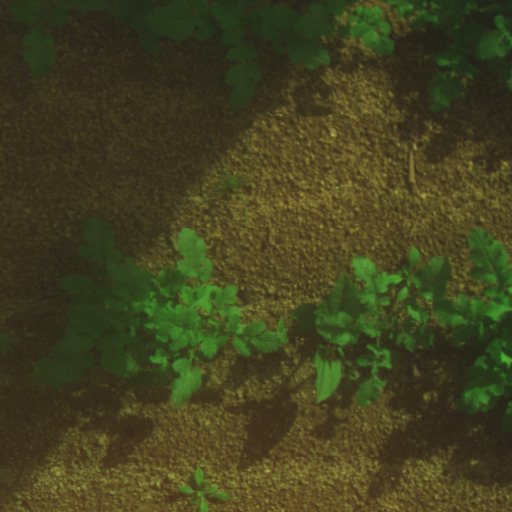
\includegraphics[width=4cm]{img/leaf/airphen-false} \nodepart{second} {\faShare*} Pre-Processing}; &
    \node (index)        [figure={blue!30}]      {\includegraphics[width=4cm]{img/leaf/airphen-index} \nodepart{second} {\faPagelines} Deep-Indices}; &
    \node (watershed)    [figure={blue!30}]      {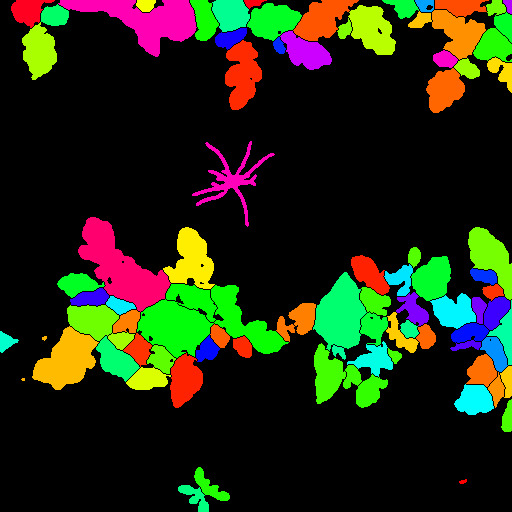
\includegraphics[width=4cm]{img/leaf/airphen-watershed} \nodepart{second} {\faLeaf} Deep-Leaves}; &
    \node (fv)    [nonterminal,rotate=90,xshift=16mm]      {{\faBolt} Optimization \\ {\faCalculator} Feature Extraction \\ {\faChartPie} And Data-Mining}; &
    %\node (cl)    [nonterminal,rotate=90,xshift=16mm]      {Classification}; &
    \node (map)    [figure={green!20}]      { \includegraphics[width=4cm]{img/conclusion/airphen-crop-weed-map} \nodepart{second} {\faSearch} Classification}; \\
};

\draw[->] (false) to (index);
\draw[->] (index) to (watershed);
\draw[->] (watershed) to (fv);
\draw[->] (fv) to (map);

\end{tikzpicture}
        \caption{Pipeline final pour la détection et la discrimination des adventices}
        \label{fig:09-global-view}
    \end{figure}
    
    La première étape du pipeline est le ``Pre-Processing'' des données, pour l'exploitation des images multispectrales acquises durant nos expérimentations. Elle consiste en la calibration de la caméra et l'utilisation d'un algorithme développé, permettant la superposition des bandes spectrales avec une erreur inférieure au pixel.
    
    La seconde étape, ``Deep-Indices'', vise à discriminer la végétation du sol. Cela consiste en l'utilisation de nouveaux indices déduis par apprentissage supervisé sur des approximateurs de fonction. Ces derniers, contrairement aux indices standards, ont l'avantage de ne pas dépendre d'une correction radiométrique. Ces Deep-Indices ont montré une nette amélioration de la qualité de la segmentation ($\SI{82.19}{mIoU}$) par rapport aux indices standards ($63.98-\SI{73.71}{mIoU}$).
    
    La troisième étape, ``Deep-Leaves'', permet d'identifier les feuilles. Un algorithme a été développé et utilise les Deep-Indices ainsi qu'un CNN qui détecte le contour des feuilles. Cette approche a montré de bonnes performances sur des jeux de données externes et sur nos données acquises en condition de terrain. Cette méthode permet de travailler avec n'importe quelle densité de feuillage et a la capacité de détecter les plus petites adventices même lors de leur émergence. % (section \ref{sec:07-discussion})
    
    %Ceci permettra une gestion ultra-localisée des adventices lors de leurs émergences, voir du phénotypage aux stades plus avancées, via une caractérisation fine du couvert végétal.
    % Des méthodes permettant de discriminer les cultures et les adventices avaient déjà été développées au sein du laboratoire, il nous avait néanmoins paru utile d'affiner ces études concernant ces algorithmes et de nouvelles méthodes ont donc été implémenté.
    
    Enfin, on réalise l'extraction des meilleures caractéristiques pour la discrimination des cultures et des adventices. Pour ce faire, on a recensé plusieurs méthodes permettant l'extraction de différents types de caractéristiques. On utilise ensuite un algorithme d'optimisation des hyperparamètres pour chacune d'elles afin de maximiser leurs performances dans notre cas d'utilisation. On termine en utilisant un algorithme de sélection de propriétés qui permet de déterminer les meilleures combinaisons des propriétés extraites.
    
    Une performance de classification de \SI{91}{\percent} a été démontrée. Nous rappelons que notre étude est à l'échelle de la feuille, ce qui est une première dans ce domaine, ainsi qu'en condition terrain. Il n'existe donc pas de points de comparaison dans la littérature. On peut cependant noter qu'à l'échelle de la plante dans différentes conditions d'acquisition, l'état de l'art \cite{Ahmed2016} donne des performances entre \SI{77}{\percent} et \SI{97}{\percent} de discrimination culture/adventices par de tels critères. Ce qui place favorablement nos résultats et offre ainsi des perspectives.
    
    % Nous avons mené notre étude en condition terrain, alors que la plupart des autres études ont été réalisées dans un laboratoire, en éclairage controler et à l'echelle de la plante. Ainsi le potentiel de discrimination de \SI{91}{\percent} présenté ici offre des perspectives intéressantes. Il a égalant été mis en exergue l'importance de l'optimisation des paramètres de certains de ces critères, ainsi que l'importance de la sélection des propriétés sur les performances.
    
    \newpage
    \section{Perspectives}
    
    \paragraph{Acquisition} Concernant la caméra, de par sa conception multi-capteurs, une méthode de recalage des bandes spectrales est nécessaire. Même si un algorithme a été développé durant cette thèse et même s'il montre d'excellentes performances pour corriger ce problème, la méthode est coûteuse en temps de calcul et il n'existe actuellement pas de solution plus performante pour cet appareil. Ainsi, bien que cette caméra offre une résolution spatiale de très bonne qualité, son utilisation ne permet pas un traitement des données en temps réel. D'autres caméras multispectrales et hyperspectrales ont vu le jour durant cette thèse, et pourraient améliorer les performances (temps de calcul ou précision). De plus, aucune correction radiométrique n'a été utilisée durant cette thèse, principalement du fait des contraintes expérimentales. Les résultats de cette thèse montrent d'excellentes performances sans cette correction radiométrique, mais l'on peut supposer qu'un tel pré-traitement les amélioreraient encore. Des approches par apprentissage profond pourraient être développées, pour proposer une correction ne nécessitant pas de dispositif d'étalonnage \cite{DBLP:journals/corr/abs-1802-00153, tian2020deep}.
    
    \paragraph{Des données synthétiques} L'annotation de larges bases de données est longue, coûteuse et souvent sujettes à des erreurs d'annotations. Dans le cas de la détection de végétation, comment définir si un pixel contient de la végétation en bordure de feuille ? Par exemple, lorsqu'il présente un mélange spectral ? Annoter précisément des images dans ce cas de figure est difficile. Certaines techniques d'augmentation de données, permettent d'ajouter de la variabilité pour ce cas de figure. Dans cette thèse, nous avons proposé d'ajouter un bruit de perlin permettant de simuler de l'ombrage. Toutefois, superposer des images ne contenant que de la végétation à des images ne contenant que du sol, en proportion variable, permettrait peut-être d'apprendre des indices encore plus résistants, mais permettrait également d'obtenir la quantité de ce mélange. Concernant les données pour la détection des feuilles, \cite{Ward2018DeepLS} a montré qu'il était possible de construire des annotations RGB synthétiques pour la détection de ces individus. Il serait fort intéressant d'étendre cette méthode à des données multispectrales en lien avec notre caméra. Pour réaliser ces données synthétiques, je propose d'utiliser soit un moteur de rendu temps-réel telque l'UnrealEngine 5 \cite{qiu2016unrealcv}, soit un moteur de rendu style path-tracing via Mitsuba 2 \cite{NimierDavidVicini2019Mitsuba2}, tous deux basés sur des rendus physiquement réalistes. En utilisant les modèles de BRDF à microfacet et les distributions GGX, différentes conditions d'acquisition et de rugosité de surface peuvent être aisément simulées. Notons de plus, que des méthodes d'informatiques graphiques permettent d'apprendre ces matériaux à partir d'un ensemble d'acquisitions \cite{dupuy2015extracting}. L'utilisation de ces technologies permettraient d'obtenir des données synthétiques d'une qualité pour l'instant inexistante dans la littérature scientifique, en agriculture de précision.
    
    \newpage
    \paragraph{Détection des individus} La détection des objets est un sujet difficile en particulier en scène dense, tel qu'il a été vu dans cette thèse. L'approche qui a été proposée ici semble prometteuse avec la conception d'une nouvelle architecture CNN, qui s'appuie sur plusieurs recherches antérieures. Bien que les résultats obtenus soient bons, des recherches complémentaires semblent nécessaires. L'échelle de la feuille semble adéquate, mais celle de la foliole serait peut-être plus facile d'un point de vue détection des objets. De plus, d'autres méthodes pourraient être ajoutées à l'architecture CNN proposée. Par exemple, l'algorithme des basins versants \cite{8099788} qui est actuellement utilisé en post-traitement (après la sortie du CNN). L'ajout d'un espace latent semble aussi prometteur d'après \cite{kulikov2018instance} pour la segmentation des feuilles. Enfin, comme nous l'avons vu, des améliorations sur la fonction de perte, et des techniques plus avancées d'augmentation des données doivent être explorée. En réalité, la construction de l'architecture d'un CNN est souvent empirique. Or, cette construction pourrait elle aussi être automatisée et améliorée à l'aide d'une optimisation des hyperparamètres. Mais cela nécessite des ressources de calcul qui n'étaient pas disponibles durant cette thèse.
    
    \paragraph{Extraction de propriétés} L'un des objectifs initiaux de la thèse était l'extraction et l'évaluation d'un ensemble de propriétés ``standards'' afin de définir leurs potentiels de discrimination pour la discrimination cultures/adventices. Il s'agissait de déterminer quels étaient les meilleurs d'entre eux. En réalité, ces caractéristiques sont fortement limitées par de nombreux facteurs. Ils ne permettent donc pas une classification parfaite. Aujourd'hui, l'apprentissage profond est la seule alternative compétitive qui pourrait permettre d'améliorer les résultats. En suivant la démarche qui a été entreprise dans cette thèse, une alternative basée sur les approximateurs de fonction est possible. On pourrait ainsi, définir les meilleures propriétés de forme à partir d'une représentation fixe du contour. De même pour les propriétés de texture et les propriétés spatiales. En réalité, un modèle type ``UNet'' synthétise déjà l'ensemble des caractéristiques de texture, de couleur et de spectre utilisables dans ce cadre de discrimination culture/adventices. De plus, les performances de l'extraction de ces caractéristiques ne permettent pas une utilisation temps réel, ce qui renforce la nécessite d'étudier l'apprentissage profond pour cette dernière étape.
    
    %Ceci permettra une gestion ultra-localisée des adventices lors de leurs émergences, voir du phénotypage aux stades plus avancées, via une caractérisation fine du couvert végétal.
    
    %\paragraph{title} Ces recherche ouvrent de nouvelles perspectives pour une gestion localisé des adventices reposant sur les feuilles. -> Phénotypage
    
    %\par Actuellement les études sur la détection des adventices par imagerie sont difficilement comparables car fortement liées aux systèmes d'imagerie, aux résolutions spatiales et au stade de développement du cycle cultural en cours. En effet, la comparaison des performances des méthodes actuelles de traitement d'images est difficile, puisque leurs études sont basées sur des critères d'appréciation disparates. C'est-à-dire que les données, les analyses et les métriques ne concordent pas entre les études. Dans la majorité des cas, elles ne permettent donc pas leurs transpositions à une nouvelle situation.
    
    %! C.Gée
    %\paragraph{Le numérique pour l'agroécologie - gestion adventices} Ces travaux seront d'une grande utilité surtout dans ce contexte de transition agroécologique où des systèmes de cultures innovants, sans recours aux herbicides, sont étudiés. Cependant, face aux aléas climatiques, aux attaques des ravageurs ou parasites, ces systèmes sont moins robustes et nécessiteront une grand réactivité pour des interventions extrêmement précises. Un suivi spatio-temporel de l'état sanitaire d'une culture avec des outils de proxi combinés aux outils de télédétection et à la modélisation permettra de prédire des tendances et d'évaluer les stress tout en identifiant les facteurs de stress. Également, pour maintenir la production agricole au regard d'une population humaine croissante (9,5 millards en 2050) tout en préservant les ressources naturelles et assurant la provision de services associés à la biodiversité des adventices (services de pollinisation, maintien de la biodiversité et des chaines trophiques basées sur les adventices). Ainsi ces outils non-destructifs issus de la proxi-détection permettront de caractériser finement la flore adventices et donc la biodiversité dans les parcelles cultivées.  Ainsi, l'innovation peut être un levier pour accompagner les agriculteurs dans la transition agroécologique.
    
    % JNP : j'ai essayé de réordonner les idées pour que ça s'enchaine davantage : Agroécologie indispensable mais sensible aux aléas. Donc caractérisation et suivi spatio-temporel pour anticiper... Donc l'innovation contribue à l'Agroécologie. 
    \paragraph{Le numérique pour l'agroécologie - gestion adventices} Ces travaux sont d'une grande utilité dans le contexte de transition agroécologique où des systèmes de cultures innovants, sans recours aux herbicides, sont étudiés. 
    En effet, ces systèmes contribueront au maintien de la production agricole et permettront de répondre aux besoins d'une population humaine croissante (9,5 millards en 2050), tout en préservant les ressources naturelles et en assurant la provision de services associés à la biodiversité des adventices (services de pollinisation, maintien de la biodiversité et des chaînes trophiques basées sur les adventices). Toutefois, ils seront moins robustes face aux aléas climatiques, aux attaques des ravageurs ou parasites, et nécessiteront une grande réactivité. 
    Face à ce problème, les outils non-destructifs issus de la proxidétection permettront de caractériser finement la biodiversité dans les parcelles cultivées. Un suivi spatio-temporel d'une parcelle avec des outils de proxidétection combinés aux outils de télédétection et à la modélisation permettra de prédire ses évolutions et d'anticiper les interventions culturales. Ainsi, l'innovation peut être un levier pour accompagner les agriculteurs dans la transition agroécologique. 
    
    %\colorbox{orange}{Je n'ai rien comrpis}
    
    %! JA V.1
    %\paragraph{Le numérique pour l'agroécologie} Ce travail nous aidera à étudier de nouvelles façons de cultiver sans utiliser d'herbicides. Cependant, si quelque chose de mal arrive aux cultures, nous devrons être très précis dans nos interventions. La surveillance de la santé des cultures à l'aide d'outils tels que la télédétection et la modélisation nous aidera à prévoir les problèmes et à déterminer les causes du stress. Cela nous permettra de maintenir une production agricole élevée tout en préservant les ressources naturelles.
    
    %! JA V.2
    
\end{document}

